\clearpage
\section{Joint PP--TG fit diagnostics}
\begin{figure}[!htbp]
\centering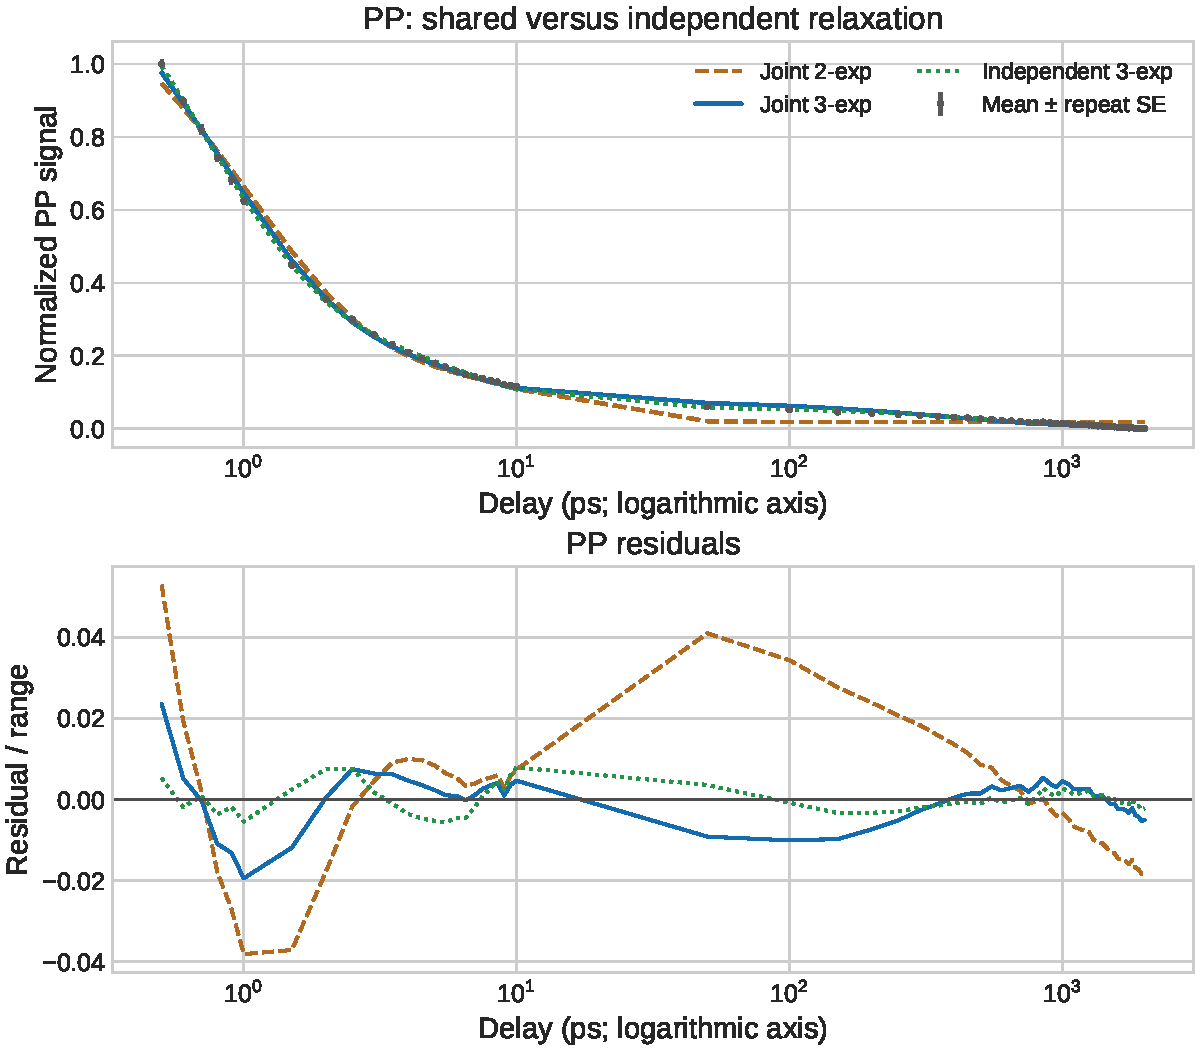
\includegraphics[width=\linewidth]{../plots/joint_pp_fit.pdf}
\caption{PP signal and residuals for the joint consistency check in Sec.~\ref{sec:joint-consistency}. The two joint fits share population lifetimes and a diffusion coefficient with all TG datasets; the independent three-exponential fit uses PP alone. The top panel subtracts the final measured mean from both data and fitted curves and divides by the fitted-window signal range for display only. Error bars are standard errors across retained repeats. Residuals use the same range normalization. The logarithmic delay axis exposes both early relaxation and the long tail. Structured residuals remain in the joint three-component model.}\label{fig:joint-pp}
\end{figure}
\FloatBarrier
\begin{figure}[!htbp]
\centering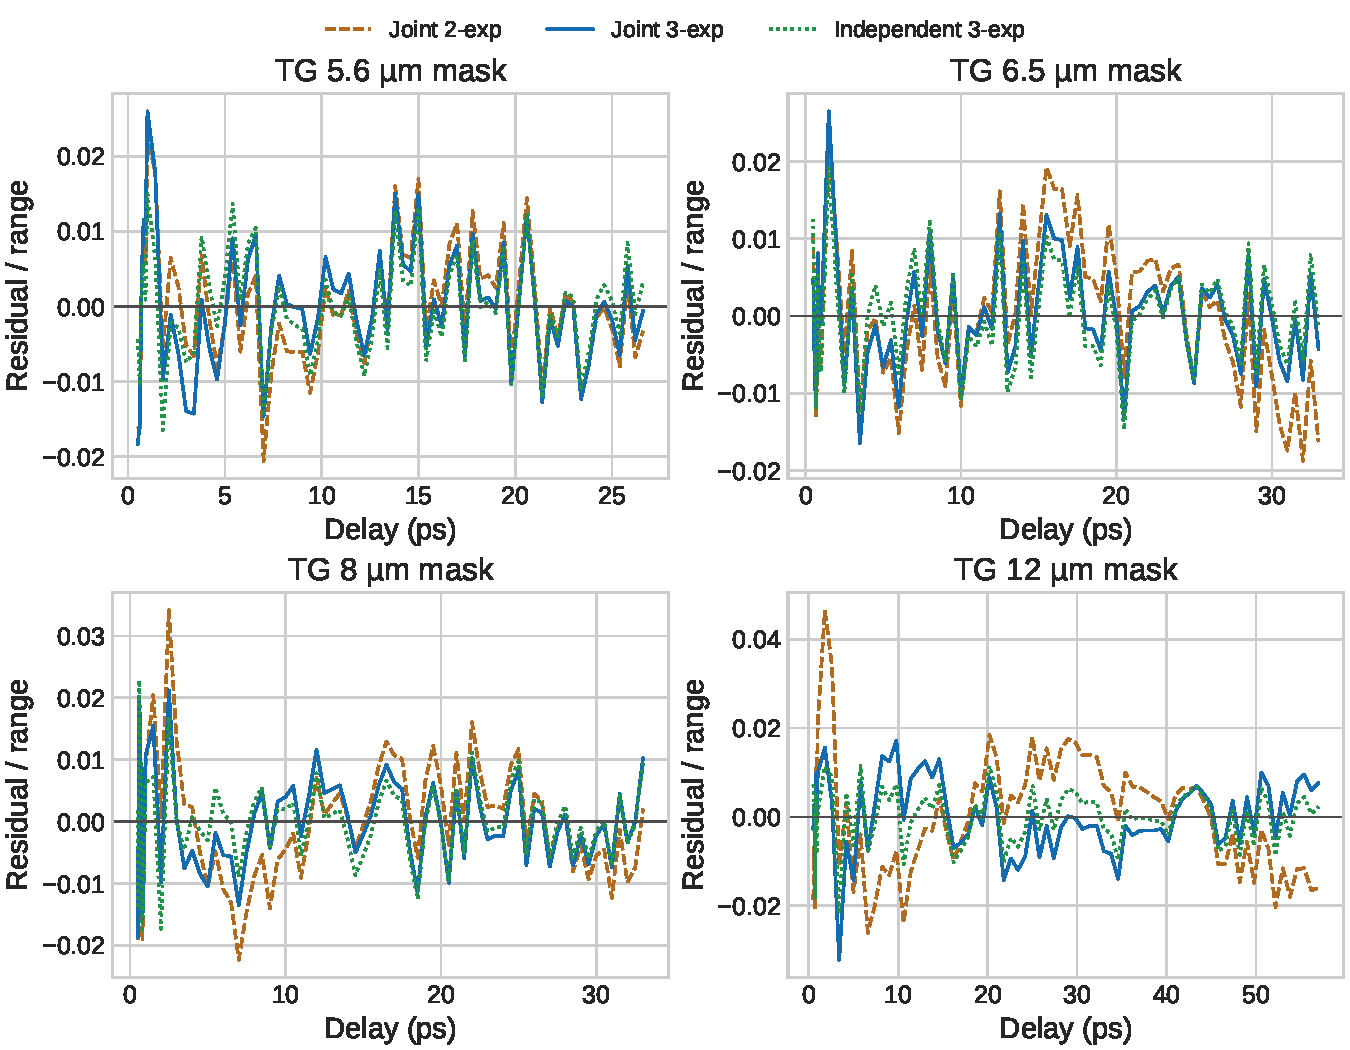
\includegraphics[width=\linewidth]{../plots/joint_tg_residuals.pdf}
\caption{TG residuals for the full-record joint two- and three-exponential models, compared with independent three-exponential fits. Each residual is the measured retained-scan mean minus the model, divided by that dataset's measured range. Each panel uses its own recorded delay interval. The third shared component improves the overall agreement, but the remaining residuals and common-window sensitivity prevent a unique physical assignment. These plots show model diagnostics, not pointwise uncertainty estimates.}\label{fig:joint-tg}
\end{figure}
\FloatBarrier
